\chapter{Data Mining}
\begin{figure}[ht!]
    \centering
    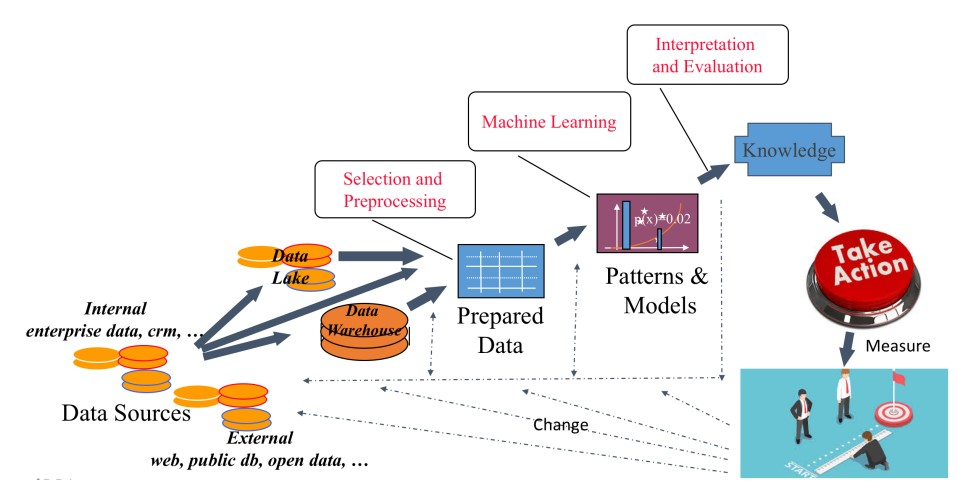
\includegraphics[scale=0.6]{images/Data_Mining_process.jpg}
    \caption{The Data Mining Process}
\end{figure}

\textbf{\textit{Data Mining}} is the process of discovering patterns, trends, correlations, or meaningful information from large datasets. It involves the application of various techniques from \textit{statistics}, \textit{machine learning}, and \textit{database systems} to extract valuable knowledge from raw data.

\section{Business Intelligence and Data Warehouses}

\textbf{\textit{Business Intelligence (BI)}} represents a key concept in the field of Data Mining and can be described as the process of:
\begin{itemize}
    \item transforming raw data into useful information to support effective and aware business strategies
    \item capturing the business data and getting the right information to the right \textit{people}, at the right \textit{time}, through the right \textit{channel}.
\end{itemize}
There are different definition that has been provided during the years, but there are two of them in particular that we can highlight:
\begin{quote}
    \textit{Business intelligence (BI) is an umbrella term that includes the applications, infrastructure and tools, and best practices that enable access to and analysis of information to improve and optimize decisions and performance. - \textbf{Gartner}}
\end{quote}
\begin{quote}
    \textit{Business Intelligence is a set of methodologies, processes, architectures, and technologies that transform raw data into meaningful and useful information used to enable more effective strategic, tactical, and operational insights and decision-making. - \textbf{Forrester Research}}
\end{quote}

One of the main tools to support BI is the \textbf{\textit{Data Warehouse (DWH)}}, which is a type of \textit{Decision Support System (DSS)} and can be seen informally as an optimized repository that stores information for the decision-making process. With the huge and increasing number of information that companies have to manage in order to find relevant business strategies DWHs answer to the necessity of more sophisticated solutions than classical operational databases.\\
The main advantages are the following:
\begin{itemize}
    \item they provide the ability to manage sets of historical data;
    \item they provide the ability to perform multidimensional analysis accurately and rapidly;
    \item they are based on a simple model that can be easily learned by its users;
    \item they are the basis for indicator-calculating systems.
\end{itemize}